\section[Cote 156-7 : supports ponctuels, ficelle à deux brins, loi orthomodulaire]{Cote 156-7 : supports ponctuels, ficelle à deux brins, loi orthomodulaire\protect\verifie[\leanblobmain]{Folder156_7}}\label{sec:156-7}

La cote 156-7, chapitre~VII de \emph{Vers une géométrie des formes}, \q{Analysis situs (troisième mouture)}, compte cent treize pages datées de sa main du 23 au 26~juin 1986. Elle reprend la notion de support de la première mouture (cote 156-4, section~\ref{sec:156-4}). Deux figures, ou deux multistrates, sont \emph{disjointes}, $X \parallel Y$ ; le \emph{cosupport} d'une partie $A$ est l'ensemble des éléments disjoints de tous ceux de $A$, le \emph{support} est le cosupport du cosupport, et un \emph{support} est une partie égale à son support (\lot{156-7}{4}{61}). Il note cette fois que \q{tout cela est formel} : il ne s'agit que d'une relation symétrique sur un ensemble. Les pages~62 et~63 en tirent les propriétés d'un treillis orthocomplémenté, celles que la section~\ref{sec:156-4} démontre pour la première mouture. Mais la page~68 ne présume plus d'algèbre de Boole. Le dossier cherche quand les supports se comportent comme des parties d'un ensemble de points (pages~72 à~80), puis rencontre deux fois le contraire : la \q{ficelle à deux brins} des pages~81 à~83, et le graphe de la page~98, qui réfute un lemme du dossier par \q{Rideau\dots}.

\noindent\emph{Conventions.} On se donne un ensemble $\mathcal M$ et une relation $\parallel$ sur $\mathcal M$. Pour $A \subset \mathcal M$, $\mathrm{cosupp}\, A = \{X \mid X \parallel Y \text{ pour tout } Y \in A\}$, $\mathrm{supp}\, A = \mathrm{cosupp}(\mathrm{cosupp}\, A)$, et l'on écrit $A \parallel B$ pour $A \subset \mathrm{cosupp}\, B$. Sur les supports, la borne inférieure est l'intersection, la borne supérieure $S \vee S' = \mathrm{supp}(S \cup S')$, et le complément est $\complement S = \mathrm{cosupp}\, S$. Une \emph{réalisation par points} est une application $X \mapsto |X|$ de $\mathcal M$ dans les parties d'un ensemble $P$, et l'on pose $|A| = \bigcup_{X \in A} |X|$.

\subsection*{Quand les supports sont des parties d'un ensemble de points}

La page~80 réunit en une Proposition ce que les pages~72 à~79 ont obtenu par morceaux, sous deux conditions (\lot{156-7}{4}{80}) :
\[
\mathrm{Supp}^1_P : \ X \parallel Y \iff |X| \cap |Y| = \varnothing , \qquad \mathrm{Supp}^2_P : \ \text{tout point } x \in P \text{ est un } |X| .
\]
La première dit que la disjonction se lit sur les points, la seconde que chaque point est le support ponctuel d'une multistrate.

\begin{encadre}
\begin{theoreme}[Grothendieck, page 80, \emph{les supports sont les parties de $P$}]
Soit $X \mapsto |X|$ une application de $\mathcal M$ dans $\mathfrak P(P)$. Sous $\mathrm{Supp}^1_P$ seule, $A \parallel B$ si et seulement si $|A| \cap |B| = \varnothing$. Sous $\mathrm{Supp}^1_P$ et $\mathrm{Supp}^2_P$, on a pour toutes parties $A, B \subset \mathcal M$
\[
|\mathrm{cosupp}\, A| = P \smallsetminus |A| , \qquad |\mathrm{supp}\, A| = |A| , \qquad \mathrm{supp}\, A = \{X \mid |X| \subset |A|\} ,
\]
$A \subset \mathrm{supp}\, B \iff \mathrm{supp}\, A \subset \mathrm{supp}\, B \iff |A| \subset |B|$, et $A \mapsto |A|$ est un isomorphisme d'ensembles ordonnés des supports sur $\mathfrak P(P)$, qui envoie le cosupport sur le complémentaire. Les supports forment donc une algèbre de Boole complète atomique, dont les atomes correspondent aux points.
\end{theoreme}
\end{encadre}

\begin{proof}
Sous $\mathrm{Supp}^1_P$, $X \in \mathrm{cosupp}\, A$ signifie que $|X|$ ne rencontre aucun $|Y|$, $Y \in A$, c'est-à-dire $|X| \cap |A| = \varnothing$. En particulier $A \subset \mathrm{cosupp}\, B$ équivaut à $|X| \cap |B| = \varnothing$ pour tout $X \in A$, soit $|A| \cap |B| = \varnothing$.

Supposons de plus $\mathrm{Supp}^2_P$. Un point de $|\mathrm{cosupp}\, A|$ est dans un $|X|$ qui ne rencontre pas $|A|$, donc hors de $|A|$. Inversement, si $x \notin |A|$, une multistrate $X$ de support $\{x\}$ est dans $\mathrm{cosupp}\, A$, et $x \in |\mathrm{cosupp}\, A|$. En appliquant cette égalité deux fois, $|\mathrm{supp}\, A| = P \smallsetminus (P \smallsetminus |A|) = |A|$, et $X \in \mathrm{supp}\, A$ signifie $|X| \cap (P \smallsetminus |A|) = \varnothing$, c'est-à-dire $|X| \subset |A|$. Il en résulte que $A \subset \mathrm{supp}\, B$ équivaut à $|A| \subset |B|$, puis, en remplaçant $A$ par $\mathrm{supp}\, A$, que $\mathrm{supp}\, A \subset \mathrm{supp}\, B$ équivaut à $|A| \subset |B|$.

Pour l'isomorphisme, on associe à $T \subset P$ la partie $\{X \mid |X| \subset T\}$. Son image par $|\cdot|$ est $T$ : chaque point de $T$ est un $|X|$ contenu dans $T$. C'est un support, puisque son support est $\{X \mid |X| \subset T\}$ par la formule précédente. Si $S$ est un support, $\{X \mid |X| \subset |S|\} = \mathrm{supp}\, S = S$. Les deux applications sont donc inverses l'une de l'autre, et $|S| \subset |S'|$ équivaut à $S \subset \mathrm{supp}\, S' = S'$. Le cosupport est envoyé sur le complémentaire par la première égalité.
\end{proof}

\begin{remarque}
La page n'écrit pas la surjectivité sur $\mathfrak P(P)$, qui vient de $\mathrm{Supp}^2_P$. Elle écrit aussi \q{$|A| = \mathrm{supp}\, A$} pour l'égalité $|A| = |\mathrm{supp}\, A|$ du Lemme~2 de la page~78. Aucune hypothèse n'est faite sur la relation $\parallel$ : la symétrie découle de $\mathrm{Supp}^1_P$, et une multistrate de support vide est disjointe d'elle-même. C'est le cas \q{particulièrement agréable} des pages~67 et~68, où la disjonction des lieux est $x \neq y$ et où les supports sont toutes les parties de $\mathcal L$.
\end{remarque}

\subsection*{La ficelle à deux brins}

La page~81 propose aussitôt un exemple où $\mathrm{Supp}^1_P$ tombe (\lot{156-7}{5}{81}). La \q{ficelle à deux brins} est formée de deux arcs qui joignent un point $0$ à un point $1$. Un lieu qui la coupe en deux est un couple de points, un sur chaque brin ; la page~82 généralise à deux ensembles totalement ordonnés $I$ et $I'$, et prend pour lieux les couples $z = (x, x') \in I \times I'$, avec le support ponctuel $|z| = \{x, x'\}$ dans la réunion disjointe $I \sqcup I'$ (\lot{156-7}{5}{82}). Deux lieux sont disjoints lorsqu'ils sont emboîtés, $z < z'$ ou $z' < z$ pour l'ordre produit ; c'est la lecture de l'édition, que la page ne décrit pas en entier, et elle rend compte de toutes ses formules.

\begin{center}
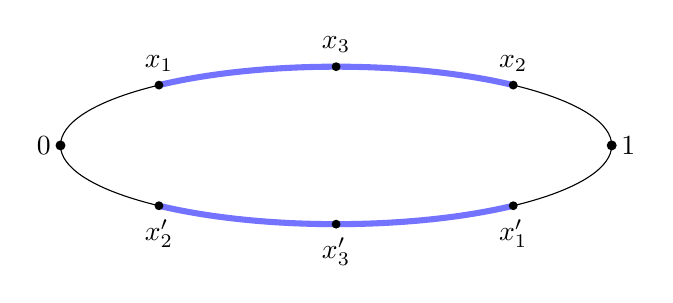
\begin{tikzpicture}[x=1cm,y=1cm]
\draw (3.5,0) ellipse (3.5 and 1);
\fill (0,0) circle (1.8pt) node[left] {$0$};
\fill (7,0) circle (1.8pt) node[right] {$1$};
\draw[line width=2.2pt, blue!55] ([shift={(3.5,0)}]130:3.5 and 1) arc[start angle=130, end angle=50, x radius=3.5, y radius=1];
\draw[line width=2.2pt, blue!55] ([shift={(3.5,0)}]230:3.5 and 1) arc[start angle=230, end angle=310, x radius=3.5, y radius=1];
\foreach \a/\n in {130/x_1,90/x_3,50/x_2} { \fill ([shift={(3.5,0)}]\a:3.5 and 1) circle (1.6pt); \node[above] at ([shift={(3.5,0.05)}]\a:3.5 and 1) {$\n$}; }
\foreach \a/\n in {230/x'_2,270/x'_3,310/x'_1} { \fill ([shift={(3.5,0)}]\a:3.5 and 1) circle (1.6pt); \node[below] at ([shift={(3.5,-0.05)}]\a:3.5 and 1) {$\n$}; }
\end{tikzpicture}
\end{center}
{\small Les lieux $z_1 = (x_1, x'_1)$ et $z_2 = (x_2, x'_2)$ se croisent ; en trait épais, $|\mathrm{supp}\{z_1, z_2\}| = [x_1, x_2] \cup [x'_2, x'_1]$, qui contient le lieu $z_3 = (x_3, x'_3)$ (d'après le dessin de la page~82).\par}
\medskip

\begin{encadre}
\begin{theoreme}[Grothendieck, pages 81 à 83, \emph{la ficelle à deux brins}]
Soient $I$ et $I'$ deux ensembles totalement ordonnés sans plus petit élément, et $J = I \times I'$, deux éléments étant disjoints s'ils sont strictement comparables pour l'ordre produit. Alors chaque $\{z\}$, $z \in J$, est un support. Soient $z_1 = (x_1, x'_1)$, $z_2 = (x_2, x'_2)$ et $z_3 = (x_3, x'_3)$ avec $x_1 < x_3 < x_2$ et $x'_2 < x'_3 < x'_1$. Alors
\[
\{z_3\} \wedge (\{z_1\} \vee \{z_2\}) = \{z_3\} , \qquad (\{z_3\} \wedge \{z_1\}) \vee (\{z_3\} \wedge \{z_2\}) = \varnothing ,
\]
et le treillis des supports n'est pas distributif. De plus $|z_1| \cap |z_2| = \varnothing$ sans que $z_1$ et $z_2$ soient disjoints, de sorte que $\mathrm{Supp}^1_P$ tombe, et $|\{z_1, z_2\}| \subsetneq |\mathrm{supp}\{z_1, z_2\}|$.
\end{theoreme}
\end{encadre}

\begin{proof}
Soit $z = (c, d)$. Son cosupport est l'ensemble des lieux strictement comparables à $z$, et $w \in \mathrm{supp}\{z\}$ signifie que $w$ est strictement comparable à chacun d'eux. Si $w$ était strictement comparable à $z$, il serait dans ce cosupport et devrait être strictement comparable à lui-même. Si $w = (a, b)$ est distinct de $z$ et incomparable, on choisit $c' < c$ et $d' < d$ ; les lieux $(c, d')$ et $(c', d)$ sont sous $z$. Comme $w$ ne majore pas $z$ et n'est pas majoré par $z$, $w$ ne peut être sous $(c, d')$ ni sous $(c', d)$, qui sont sous $z$. Il est donc au-dessus des deux, d'où $c \leq a$ et $d \leq b$, et $z \leq w$, ce qui est exclu. Ainsi $\mathrm{supp}\{z\} = \{z\}$.

Soit $u$ strictement comparable à $z_1$ et à $z_2$. S'il est sous $z_1$ et au-dessus de $z_2$, sa première coordonnée est $\leq x_1$ et $\geq x_2$, ce qui contredit $x_1 < x_2$ ; de même pour l'autre cas croisé, sur le second brin. Il est donc sous les deux, et alors $u \leq (x_1, x'_2)$, strictement sous $z_3$ ; ou au-dessus des deux, et alors $u \geq (x_2, x'_1)$, strictement au-dessus de $z_3$. Donc $z_3 \in \mathrm{supp}\{z_1, z_2\} = \{z_1\} \vee \{z_2\}$, ce qui donne la première égalité. Pour la seconde, $\{z_3\} \cap \{z_1\} = \{z_3\} \cap \{z_2\} = \varnothing$, et le support du vide est le cosupport de $J$ tout entier, qui est vide puisque aucun lieu n'est disjoint de lui-même. Enfin $|z_1| = \{x_1, x'_1\}$ et $|z_2| = \{x_2, x'_2\}$ sont disjoints, alors que $z_1$ et $z_2$ sont incomparables. Le point $x_3$ de $|z_3|$ est dans $|\mathrm{supp}\{z_1, z_2\}|$ et hors de $|\{z_1, z_2\}| = \{x_1, x_2, x'_1, x'_2\}$.
\end{proof}

\begin{remarque}
La page~82 donne à $I$ et à $I'$ des extrémités, la page~81 prend pour lieux intérieurs $]0,1[ \times ]0,1[$. L'énoncé démontré porte sur les lieux intérieurs ; les lieux $0$ et $1$, de supports $\{0\}$ et $\{1\}$, sont laissés de côté. Ni la densité ni les extrémités ne servent ; il suffit que les brins n'aient pas de plus petit élément, et sans cette hypothèse $\{z\}$ peut cesser d'être un support. Dans le produit de deux chaînes à trois éléments $0 < 1 < 2$, le support de $\{(0, 2)\}$ contient $(1, 1)$ (vérifié en Lean par énumération). La page écrit enfin \q{on n'a pas la propriété modulaire}, suivi d'un mot non lu, à côté de la distributivité. L'exemple réfute la distributivité ; on ne dit rien ici de la modularité.
\end{remarque}

\subsection*{Le lemme de la page 97, réfuté page 98}

Pour démontrer un théorème sur les intérieurs des multistrates (page~93), il le ramène à un énoncé formel sur une relation symétrique antiréflexive, puis, page~97, au \emph{Lemme~3} : si $S$ et $S'$ sont des supports et $S \parallel S'$, alors $S' = (S \vee S') \cap \complement S$. Une marge écrit \q{Faux} (\lot{156-7}{5}{97}). La page suivante donne la raison : \q{Mais c'est faux ! Prenons p.~ex.\ un graphe [\dots] ($A$ et $B$ ne sont liés qu'aux sommets $A'$, $B'$ et entre eux)}, et conclut \q{Rideau\dots} (\lot{156-7}{5}{98}). La disjonction y est la relation \q{être liés} du graphe.

\begin{center}
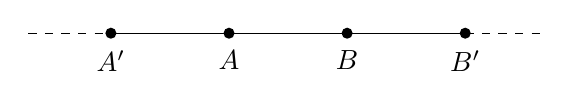
\begin{tikzpicture}[x=1.5cm,y=1cm]
\draw[dashed] (-0.7,0) -- (0,0);
\draw[dashed] (3,0) -- (3.7,0);
\draw (0,0) -- (1,0) -- (2,0) -- (3,0);
\foreach \x/\n in {0/A',1/A,2/B,3/B'} { \fill (\x,0) circle (2pt); \node[below] at (\x,-0.1) {$\n$}; }
\end{tikzpicture}
\end{center}
{\small Le graphe de la page~98 ; les pointillés prolongent le graphe au-delà de $A'$ et de $B'$. Le modèle vérifié est la chaîne de quatre sommets.\par}
\medskip

\begin{encadre}
\begin{contrexemple}[Grothendieck, pages 97 et 98, \emph{la loi orthomodulaire tombe}]
Sur la chaîne $A' - A - B - B'$, deux sommets étant disjoints s'ils sont liés, on a $\mathrm{cosupp}\{A\} = \{A', B\}$, $\mathrm{supp}\{A\} = \{A\}$, $\mathrm{cosupp}\{B\} = \{A, B'\}$, $\mathrm{supp}\{B\} = \{B\}$. Les supports $S = \{A\}$ et $S' = \{B\}$ sont disjoints, $S \vee S' = \mathcal M$, et
\[
(S \vee S') \cap \complement S = \{A', B\} \neq S' .
\]
Les supports sont exactement $\varnothing$, $\{A\}$, $\{B\}$, $\{A', B\}$, $\{A, B'\}$ et $\mathcal M$.
\end{contrexemple}
\end{encadre}

\begin{proof}
Le cosupport d'un sommet est l'ensemble de ses voisins, et le cosupport d'une partie l'ensemble des voisins communs à tous ses sommets. Les voisins communs de $A'$ et de $B$ se réduisent à $A$, ceux de $A$ et de $B'$ à $B$. Aucun sommet n'est voisin à la fois de $A$ et de $B$, donc $\mathrm{cosupp}\{A, B\} = \varnothing$ et $S \vee S' = \mathrm{cosupp}\, \varnothing = \mathcal M$. Alors $(S \vee S') \cap \complement S = \{A', B\}$. En Lean, ces calculs et la liste des seize parties qui sont des supports sont vérifiés par énumération exhaustive dans le noyau.
\end{proof}

\begin{remarque}
Le Lemme~3 est la \emph{loi orthomodulaire} : pour $S' \leq \complement S$, $S' = (S \vee S') \wedge \complement S$. Le graphe de la page~98 est le graphe de disjonction du modèle à sept éléments de la section~\ref{sec:156-4} : les paires disjointes y sont $\{a, b\}$, $\{b, c\}$, $\{c, d\}$, la chaîne $a - b - c - d$, et ses parties saturées $\varnothing$, $\{b\}$, $\{c\}$, $\{a, c\}$, $\{b, d\}$, $\mathcal M$ sont celles de la chaîne, avec $A = b$ et $B = c$. Le graphe qui réfute dans l'édition la présomption d'une algèbre de Boole de la première mouture est donc celui que Grothendieck trouve lui-même, deux semaines plus tard, contre son propre lemme. La conclusion est plus forte : ce treillis hexagonal, l'orthotreillis classique à six éléments, n'est même pas orthomodulaire. La page~98 ne renonce pas : la formule $S_{A \smallsetminus B} = S_A \cap \complement S_B$ devrait être vraie, écrit-il, \q{du moins sous l'hypothèse de divisibilité At\,L1}.
\end{remarque}

Ne sont pas démontrés ici : les axiomes de l'atelier (pages~1 à~60) et l'identification de $\Sigma_{\mathfrak F}$ à $\Sigma_{\mathcal M}$ (page~61) ; le changement d'ensemble de référence $\Lambda$ (pages~64 à~68) ; les Lemmes des pages~76 à~79 sous les seules hypothèses (iii)$_{\mathcal M}$, (vi\,a)$_{\mathcal M}$ et Hyp. ; l'unicité de $P$ annoncée page~81 ; le théorème de la page~93 sur les intérieurs et ce que la page~98 espère sous At\,L1 ; les magasins (pages~101 à~113).
